\section{Introduction}
Among all features of the human body, many may be employed to authenticate and authorize people by making use of the incredible natural diversity in human appearances. 
Fingerprints in particular, stand out as one of the most reliable methods to identify individuals.
Increased availability, compactness and convenience of modern digital capture systems have long surpassed analog methods in speed for everyday usage.

With all these benefits, some problems, such as unsupervised incorrect authorizations, can have catastrophic outcomes.
The human skin hones many imperfections and, over time, rarely stays in the original condition it was captured in.
As a result, some tolerance is needed between the original and a recent fingerprint capture to prevent access denials in situations where fingers may be wet, dirty, or damaged.
Advancements in fingerprint pattern replacements have resulted in them being almost indistinguishable from bona fide fingerprints when the aforementioned tolerance is considered.
Additional protection against artificially constructed fingerprint images is needed in the form of liveliness detection systems which determine whether a presented fingerprint originates from a live human or not.

Malicious intent is often connected to high-value targets like critical infrastructure or border control systems, and successful intrusions can lead to severe consequences.
These authentication systems are operating with high accuracy and no tolerance for errors, which requires specialized and costly hardware.
High-quality fingerprint scanners are challenging to integrate into systems such as smartphones and personal computers, nonetheless representing targets for unauthorized access.

Restricted space and aggressive cost optimization create the need for small capture devices which are easy to use, easy to integrate, and cheap to produce. 
The reduction in capture-device quality naturally comes with a reduction in authentication accuracy.
Software-enhanced authentication systems can deliver impressive results while not requiring complex capture devices.



\subsection{Neural Networks}
Open-Source libraries such as \gls{keras} offer simple interfaces for complicated software frameworks and provide ready-to-use machine learning implementations.
Following experiments are conducted using a selection of pre-trained deep learning models from \gls{keras} using \gls{tensorflow} as the underlying platform.

Spacial diversity was a category for selecting the algorithms to give insight on how complicated a deep learning network needs to be to provide confident decisions on whether a presented fingerprint image is coming from a live person or not.
It is important to note that these networks are image classifiers coarsely detecting the image's contents.
The classifier MobileNet, for example, can detect real-world objects and animals and is intended for "mobile and embedded vision applications" \cite{MBNET}.
All networks are pre-trained on the ImageNet dataset containing "1000 object classes and [...] 1,281,167 training images" \cite{ImageNet}. 


\begin{tabular}{| l | r | r |}
    \hline
    Network Name   & Size    & Parameters \\ \hline\hline
    MobileNet      & 16 MB   &   4,253,864 \\ \hline
    NASNetMobile   & 23 MB   &   5,326,716 \\ \hline
    EfficientNetB0 & 29 MB   &   5,330,571 \\ \hline\hline
 
    Xception       & 88 MB   &  22,910,480 \\ \hline
    InceptionV3    & 92 MB   &  23,851,784 \\ \hline
    EfficientNetB5 & 118 MB  &  30,562,527 \\ \hline\hline

    NASNetLarge    & 343 MB  &  88,949,818 \\ \hline
    VGG16          & 528 MB  & 138,357,544 \\ \hline
    VGG19          & 549 MB  & 143,667,240 \\ \hline
\end{tabular}
\caption{Table: Neural Networks}


A total of nine different neural networks were categorized by their size and depth into three groups (see Table \ref{tbl:nerual_networks}).
Each network was custom fitted into the task at hand with wrapper-layer encapsulating the intended behavior in a non-intrusive way to ensure that the default behavior is sustained.
Each neural networks' internal behavior is treated as a black box.

The original input layer was discarded and replaced with a generic Input Layer accepting images of size 250x250. All models share the same input layer implementation.
Furthermore, two additional layers were added to the stack to flatten the neural network's output and to result in a liveliness prediction score between $0$ and $1$.
Sigmoid is used as the activation function.

It seems intuitive that complex networks should outperform lightweight implementations when comparing the validation accuracy, as the increased number in parameters gives an advantage.
However, training times and prediction latencies are also expected to increase with a higher parameter count.


% fig: cnn composition

\subsection{Dataset}
The provided fingerprint samples were originally used as input material for a conference and competition about fingerprint detection.
Bona fide fingerprints of 54 individuals were captured five times, summing up to 2700 genuine fingerprints.
For a subset of individuals, an artificial fingerprint was crafted using multiple materials to create a set of fake images adding up to 3740 fake fingerprint images.



    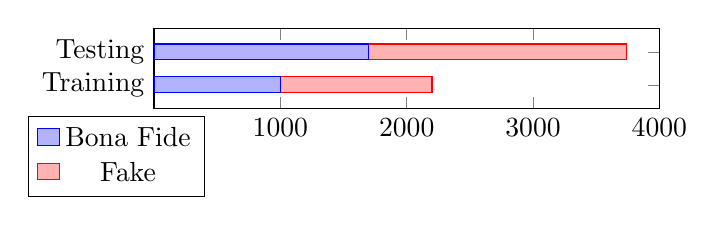
\begin{tikzpicture}
        \begin{axis}[
            xbar stacked, xmin=0, xmax=4000,
            width=8cm,height=2.6cm,
            bar width=2mm,
            xtick={1000,2000,3000,4000},
            xticklabels={1000, 2000, 3000, 4000},
            symbolic y coords={Training,Testing},
            ytick=data,enlarge y limits={abs=3mm},
            legend style={
                at={(-0.25,-0.6)},
                anchor=west,
            }
        ]
            \addplot coordinates { (1000,{Training}) (1700,{Testing})};
            \addplot coordinates { (1200,{Training}) (2040,{Testing})};
            \legend{Bona Fide, Fake}
        \end{axis}
    \end{tikzpicture}

\vspace{-8mm}
\caption{Fingerprint Image Count}
\label{fig:dataset}
\begin{table}[htb]
    \centering

    \begin{minipage}[r]{0.25\textwidth}
        \centering Training Data (37\%)
        
        \smallskip
        \begin{tabular}{ l r } \hline
            Material    & Share \\ \hline
            Live        & 45\%  \\
            Body Double & 18\%  \\
            Ecoflex     & 18\%  \\
            Wood Glue   & 18\%  \\ \hline
        \end{tabular}
    \end{minipage}
    \hspace{10mm}
    \begin{minipage}[r]{0.25\textwidth}
        \centering Testing Data (63\%)
        
        \smallskip
        \begin{tabular}{ l r } \hline
            Material        & Share \\ \hline
            Live            & 45\%  \\
            Gelatine        & 18\%  \\
            Latex           & 18\%  \\
            Liquid Ecoflex  & 18\%  \\ \hline
        \end{tabular}
    \end{minipage}

    \caption{Material Distribution}
\end{table}



Machine learning algorithms get more accurate the more data for training purposes is provided, as a richer set of unique training input improves the networks prediction skills.
The popular machine learning utility library \gls{sklearn} splits the data into training and validation subsets with a ratio of 3:1 \cite{sklearn}.
For the LivDet2017 dataset, the ratio is almost flipped, with only 37\% of images used for training purposes.
As illustrated in Figure \ref{fig:dataset} and Table \ref{tbl:dataset_materials} the training dataset is approximately 50\% smaller than the validation dataset.

About half (45\%) of each dataset are bona fide fingerprints and the other half is comprised of materials emulating human skin.
Body Double, Ecoflex, and Wood Glue (each 18\%) were used to train while Gelatine, Latex, and Liquid Ecoflex (also each 18\%) are used for validation.
59\% of fingerprint samples are from female subjects while 41\% are from males.
Each image was also classified with an age.



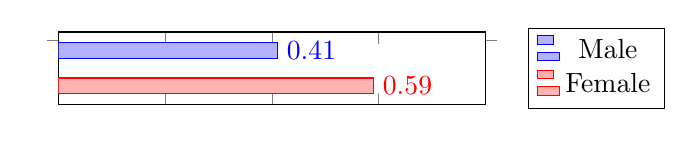
\begin{tikzpicture}
    \begin{axis}[
        xbar, xmin=0, xmax=0.8,
        width=7cm,height=2.5cm,
        bar width=2mm,
        symbolic y coords={F,M},
        ytick=data,enlarge y limits={abs=1mm},
        nodes near coords,
        yticklabels={,},
        xticklabels={,},
        legend style={
            at={(1.1,0.5)},
            anchor=west,
        }
    ]
        \addplot coordinates { (0.41,{M}) };
        \addplot coordinates { (0.59,{F}) };
        \legend{Male, Female}
    \end{axis}
\end{tikzpicture}
\vspace{-5mm}
\caption{Sex Distribution}
\begin{tikzpicture}
    \begin{axis}[
        height=25mm,
        width=95mm,
        yticklabels={},
        xtick={21, 25, 31.3, 40, 77},
        xticklabels={21, 25, 31.3, 40, 77}]

        \addplot+ [
            boxplot prepared={
                box extend=0.6,
                whisker extend=1,
                lower whisker=19.0, 
                lower quartile=21.0,                
                median=25.0,
                upper quartile=40.0,
                upper whisker=77.0,
                average=31.3
            }
        ] coordinates {};
    \end{axis}
\end{tikzpicture}
\vspace{-2mm}
\caption{Age Distribution}
\label{img:age-dist}


No recognizable variance in prediction accuracy is expected as the difference in sex and age do not infer a significant change in fingerprint anatomy or appearance to play a role in this experiment.
With that said, a more mature finger can have noticeable damage like scars or common wear from labor and general use.

All images were captured on a Green Bit DactyScan84C and have a resolution of 500x500 pixel.
The scanner is a standalone high-end device capturing fingerprints in high resolution.
Bona fide fingerprint images are of such high quality that sweat glands are visible as small white spots on fingerprint ridges in some samples as illustrated in Figure \ref{fig:sweat-glands}.

Important to note is that none of the used material groups share distinct properties or features.
It is, therefore, more difficult for the trained algorithms to infer the artificiality of unknown materials.

Below is a fingerprint image from each material group (see Figure \ref{fig:fake_fingers}).
None of the materials capture sweat glands which may be beneficial to determine whether the presented image is an a attack presentation or genuine.

The images used in the context of the experiments are only a subset of the dataset used in the LivDet 2017 competition.

\begin{minipage}[r]{0.5\textwidth}
    \begin{minipage}[r]{0.3\textwidth}
        \centering
        \includegraphics[width=\linewidth]{fake-ecoflex.bmp}
        \vspace{-10mm}\caption{Ecoflex}
    \end{minipage}
    \begin{minipage}[r]{0.3\textwidth}
        \centering
        \includegraphics[width=\linewidth]{fake-body-double.bmp}
        \vspace{-10mm}\caption{Body Double}
    \end{minipage}
    \begin{minipage}[r]{0.3\textwidth}
        \centering
        \includegraphics[width=\linewidth]{fake-wood-glue.bmp}
        \vspace{-10mm}\caption{Wood Glue}        
    \end{minipage}
    \caption{Training Dataset}
\end{minipage}
\vrule
\begin{minipage}[r]{0.5\textwidth}
    \begin{minipage}[r]{0.3\textwidth}
        \centering
        \includegraphics[width=\linewidth]{fake-gelatine.bmp}
        \vspace{-10mm}\caption{Gelatine}
    \end{minipage}
    \begin{minipage}[r]{0.3\textwidth}
        \centering
        \includegraphics[width=\linewidth]{fake-latex.bmp}
        \vspace{-10mm}\caption{Latex}
    \end{minipage}
    \begin{minipage}[r]{0.3\textwidth}
        \centering
        \includegraphics[width=\linewidth]{fake-liquid-ecoflex.bmp}
        \vspace{-10mm}\caption{Liquid-Ecoflex}        
    \end{minipage}
    \caption{Validation Dataset}
\end{minipage}


\subsection{Methodology}
The experiment is split into two parts.
During the first phase, the best-case (highest average validation accuracy) for each network is determined.
Due to randomized initial values and subsequent variance in training evolution, the resulting validation accuracy can fluctuate to some degree.
Repetitive training and evaluation will give sets of models for each network that can be serialized and stored.

All model-internal layers are initially frozen to inspect out-of-the-box behavior while training with the same procedure once more.
During the second training, all parameters are unfrozen and able to change.
A comparison between default and more specialized models will give insight into the importance of adaptive training.
The unfrozen models are expected to perform a lot better.

Models are compiled with an Adam-Optimizer using a learning rate of 0.0001 and a binary cross-entropy loss function.
Models are trained using the provided training dataset over ten epochs, which delivered a good balance between validation accuracy and training time.
At that point training accuracy was at 100\% and the loss value fluctuated around the training sessions minimum.

A total of ten training iterations for each network will be used as a pool to pick the best-performing model.

Trained models are not volatile, so using the best case for each is the fairest approach to ensure every network has the best chances.

Further experiments are conducted in the second phase, where the best-case models for each network predict whether a fingerprint presentation is bona fide or an artificially constructed fingerprint replica.
Unlike neural network training, the predictions of the trained model are static and will not change.
The resulting predictions are used to analyze possible correlations between input data and predicted values.

Predictions are classified by assuming that prediction values of at least 0.50 suggest a bona fide fingerprint while all lower values suggest an attack presentation.
This ratio was chosen to directly compare scores and accuracies with ones from the algorithms submitted to the conference. \cite{LIVDET}
Since the activation function producing the scores is sigmoid, the prediction confidences are concentrated at the two extrema leaving few indecisive predictions.
% show graph about prediction confidence scatter

Various aggregates will show possible correlations in prediction accuracy between the used material in case of a presentation attack or otherwise prediction differences in sex and age of the test subject.
Additionally, the prediction latency for each network will be discussed and brought into context with the networks' size and complexity.


All experiments are performed on a capable workstation with an 8/16 Core CPU, 16Gb RAM and discrete graphics.
TensorFlow reports a compute capability of $6.1$.
The hardware does not have an impact on prediction accuracy but rather training and prediction times.